\documentclass{article}
\usepackage{graphicx}
\usepackage{caption}
\usepackage{polski}
\usepackage[utf8]{inputenc}
\usepackage{listings}
\graphicspath{{./pics}}
\title{Rozwiązania testu - Projektowanie i wdrażanie systemów w chmurze}
\author{Mateusz Zając (298654)}

\usepackage{color}
\definecolor{lightgray}{rgb}{.9,.9,.9}
\definecolor{darkgray}{rgb}{.4,.4,.4}
\definecolor{purple}{rgb}{0.65, 0.12, 0.82}

\lstdefinelanguage{JavaScript}{
	keywords={typeof, new, true, false, catch, function, return, null, catch, switch, var, if, in, while, do, else, case, break},
	keywordstyle=\color{blue}\bfseries,
	ndkeywords={class, export, boolean, throw, implements, import, this},
	ndkeywordstyle=\color{darkgray}\bfseries,
	identifierstyle=\color{black},
	sensitive=false,
	comment=[l]{//},
	morecomment=[s]{/*}{*/},
	commentstyle=\color{purple}\ttfamily,
	stringstyle=\color{red}\ttfamily,
	morestring=[b]',
	morestring=[b]"
}

\lstset{
	language=JavaScript,
	backgroundcolor=\color{lightgray},
	extendedchars=true,
	basicstyle=\footnotesize\ttfamily,
	showstringspaces=false,
	showspaces=false,
	numbers=left,
	numberstyle=\footnotesize,
	numbersep=9pt,
	tabsize=2,
	breaklines=true,
	showtabs=false,
	captionpos=b
}


\begin{document}
	\maketitle
	\section*{Zadanie 1}
		\begin{figure}[h!]
			
\includegraphics[width=1\textwidth]{za1}
		\end{figure}
		Żeby potwierdzić tę hipotezę, muszę przyjrzeć się odpowiedniemu nagłówkowi HTTP i zweryfikować jego zawartość. W tym celu muszę mieć możliwość obejrzenia poszczególnych zapytań HTTP, na przykład tak:
		\begin{enumerate}
			\item \textbf{Użycie Postmana i przejrzenie zapytań wysyłanych przez przeglądarkę.} 
			
			Aplikacja Postman posiada rozszerzenie do przeglądarki Google Chrome, która po aktywacji zapisuje zapytania HTTP w historii zapytań aplikacji. Po wejściu na stronę Google historia zapytań wygląda tak:
			\begin{figure}[h!]
				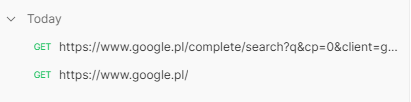
\includegraphics[width=1\textwidth]{googlehttp}
			\end{figure}
			\clearpage
			Możemy podejrzeć nagłówek zapytania:
			\begin{figure}[h!]
				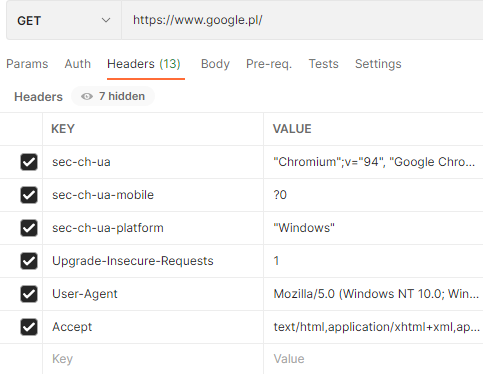
\includegraphics[width=1\textwidth]{googlehttpdetails}
			\end{figure}
			
			\item \textbf{Użycie curl}
			
			Możemy również użyć programu "curl" w konsoli linuxowej. Jeśli chcę podejrzeć wysyłane nagłówki zapytania np. do http://www.google.pl, mogę wywołać curl w ten sposób: \texttt{curl -v http://www.google.pl}.
			Dzięki temu zobaczę wszystkie nazwy nagłówków oraz ich zawartość:
			\begin{figure}[h!]
				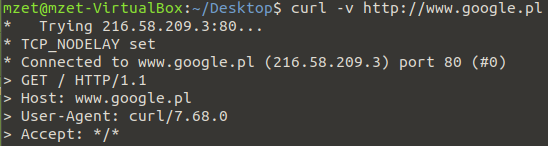
\includegraphics[width=1\textwidth]{curlhttp}
			\end{figure}
		
			\item \textbf{Sprawdzenie pakietów przy pomocy narzędzi deweloperskich Google Chrome}
			
			Alternatywnie, mogę użyć wbudowanych narzędzi deweloperskich przeglądarki Google Chrome, aby podejrzeć wysyłane zapytania. Mogę tutaj podejrzeć zarówno zapytanie, jak i odpowiedź na nią.
			\begin{figure}[h!]
				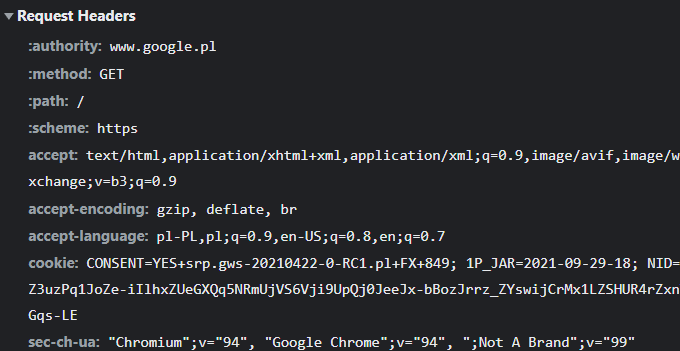
\includegraphics[width=1\textwidth]{chromereq}
			\end{figure}
			 
		\end{enumerate}	
	\section*{Zadanie 2}
		\begin{figure}[h!]
			
\includegraphics[width=1\textwidth]{za2}
		\end{figure}
	
		Najszybszym i najprostszym sposobem na transfer dużej ilości plików w bezpieczny sposób przez sieć jest użycie protokołu SFTP. Jeśli na serwerze jest włączona ta usługa, mogę się do niego zdalnie podłączyć, używając menedżera FTP (np Filezilla lub Total Commander). Po prostu podaję adres serwera, loguję się i mogę swobodnie transferować pliki z obie strony. Mogę też edytować pliki bezpośrednio na serwerze.
		
		Aby uruchomić program na serwerze zdalnym oraz wykonywać komendy, mogę użyć SSH. Tam także wystarczy podanie adresu serwera oraz zalogowanie. Od tej chwili mogę korzystać z konsoli serwerowej na komputerze lokalnym.
		
		Innym rozwiązaniem, bez użycia SFTP może być komenda \texttt{scp}. Służy do bezpiecznego kopiowania plików z lokalnego komputera na serwer. Lepszym rozwiązaniem jest natomiast użycie \texttt{rsync}, który robi to szybciej i sprawniej.
		
		Jeśli nad kodem aplikacji pracuje więcej osób, należy rozważyć użycie repozytorium kodu (np. Git) wraz z synchronizacją kodu serwera z kodem repozytorium (takie rozwiązaniem stosuje np. Heroku).
		\newpage
	
	\section*{Zadanie 3}
		\begin{figure}[h!]
			
\includegraphics[width=1\textwidth]{za3}
		\end{figure}
	
		Należy sprawdzić, jaki stan ma ten port na serwerze. Możemy to zrobić przy pomocy \texttt{netstat} (w konsoli serwera). Potem od razu filtrujemy wynik narzędziem \texttt{grep}:
		\texttt{netstat | grep "5678"}.
		Jeśli nastąpi jakiś problem (port, który wybraliśmy nie ma statusu "LISTEN"), oznacza to, że mamy problem z nasłuchiwaniem na tym porcie. Być może inna aplikacja z niego korzysta lub nasz program nie ma uprawnień do zajęcia portu.
		
		Bezpośrednim sprawdzeniem czy mamy połączenie z adresem serwera na danym porcie jest wywołanie:
		\texttt{telnet (adresserwera) (port)}.
		Jeżeli uda nam się poprawnie połączyć, po stronie sieci nie ma problemów z połączeniem. Problem może leżeć w aplikacji.
		
		Jeśli natomiast nie możemy się połączyć, sprawdzić musimy także, czy nasza brama sieciowa (np. router, który łączy serwer z internetem) umożliwia łączenie na tym porcie. Możemy to sprawdzić w ustawieniach bezpieczeństwa na urządzeniu sieciowym. Potrzebnym może być dodanie wyjątku w zaporze sieciowej urządzenia.
		
	\section*{Zadanie 4}
		\begin{figure}[h!]
			
\includegraphics[width=1\textwidth]{za4}
		\end{figure}
		Najprostszym dla mnie sposobem na stworzenie tego serwera jest napisanie prostej aplikacji w \texttt{Node.js} przy pomocy frameworka \texttt{Express}. Mogę szybko zdefiniować ścieżki, na które ma reagować serwer, a dzięki bibliotece standardowej javaScript mogę wyciągnąć potrzebne informacje o czasie i pamięci maszyny:
		
		\begin{lstlisting}
			// Mateusz Zajac
			// 298654
			// Projektowanie i wdrazanie systemow w chmurze
			
			const express = require('express')
			const app = express()
			const port = 1234
			const os = require('os')
			
			var lastVal = ""
			
			// This path prints the current server time
			app.get('/index', (req, res) => {
				var mytime = new Date(Date.now())
				res.send(`My current time is: ${mytime}`)
			})
			
			// This path prints free memory in Megabytes
			app.get('/test/test1', (req, res) => {
				// It returns number in bytes, 
				// i want to cast it to MB for readability,
				//  therefore division by 1e6
				var freemem = os.freemem/(1e6)
				res.send(`My free memory: ${parseInt(freemem)}MB`)
			})
			
			// This path sets lastVal variable to "George has a cat"
			app.get('/test/test2', (req, res) => {
				lastVal = "George has a cat"
				res.redirect("/przyklad")
			})
			
			// This path sets lastVal variable to "Cat has George"
			app.get('/test/test3', (req, res) => {
				lastVal = "Cat has George"
				res.redirect("/przyklad")
			})
			
			// This path prints lastVal variable on the screen
			app.get('/przyklad', (req, res) => {
				res.send(`My last value is: ${lastVal}`)
			})
			
			// This one runs the whole app on port 1234
			// And prints the message to confirm it
			app.listen(port, () => {
				console.log("I'm ready!")
			})
		\end{lstlisting}
		Napisanie całości zajmuje około godzinę (uzwględniając instalację \texttt{Node.js}, frameworku \texttt{Express} oraz inicjalizację projektu za pomocą \texttt{npm init}).
\end{document}